\documentclass[11pt,letterpaper]{article}

% include figures
\usepackage{graphicx}
% get nice colors
\usepackage{xcolor}

% change default font to Palatino (looks nicer!)
\usepackage[latin1]{inputenc}
\usepackage{mathpazo}
\usepackage[T1]{fontenc}
% load some useful math symbols/fonts
\usepackage{latexsym,amsfonts,amsmath,amssymb,wasysym}
% be able to insert code
\usepackage{listings}

% comfort package to easily set margins
\usepackage[top=1in, bottom=1in, left=1in, right=1in]{geometry}

% spacing after a paragraph
\setlength{\parskip}{.15cm}
% indentation at the top of a new paragraph
\setlength{\parindent}{0.0cm}


\begin{document}

\begin{center}
\Large
Ay190 -- Worksheet 6\\
Daniel DeFelippis\\
Date: \today
\end{center}

%%
%%
%% I worked with Scott Barenfeld
%%
%% All python code can be found in the ws6 directory in my repository
%%
%%

\section{The Discrete Fourier Transform}

In this worksheet, we compare the performance of a function to compute a
discrete fourier transform by matrix multiplication and NumPy's fast fourier
transform. Surprise, surprise: NumPy's is much faster.

\subsection*{a}

My dft function is shown below. 
\lstinputlisting[language=Python, firstline=3]{dft.py}

We compare that function to NumPy's own fft function with the code
\lstinputlisting[language=Python, firstline=14, lastline=16]{ws6.py}
and the resulting two arrays are indeed identical. 

\subsection*{b}

Using the code from the worksheet, we can plot the time it takes to do 
100 fourier transforms on random matrices of sizes $N = 10$ to $100$.
I chose 100 fourier transforms for each value of N so that the resulting plot 
looks smoother, but it also doesn't take to long to run.

Shown below in figure~\ref{fig:6b} is a graph of the time vs the matrix size for my
transform function and NumPy's transform function. 

\begin{figure}[bth]
\centering
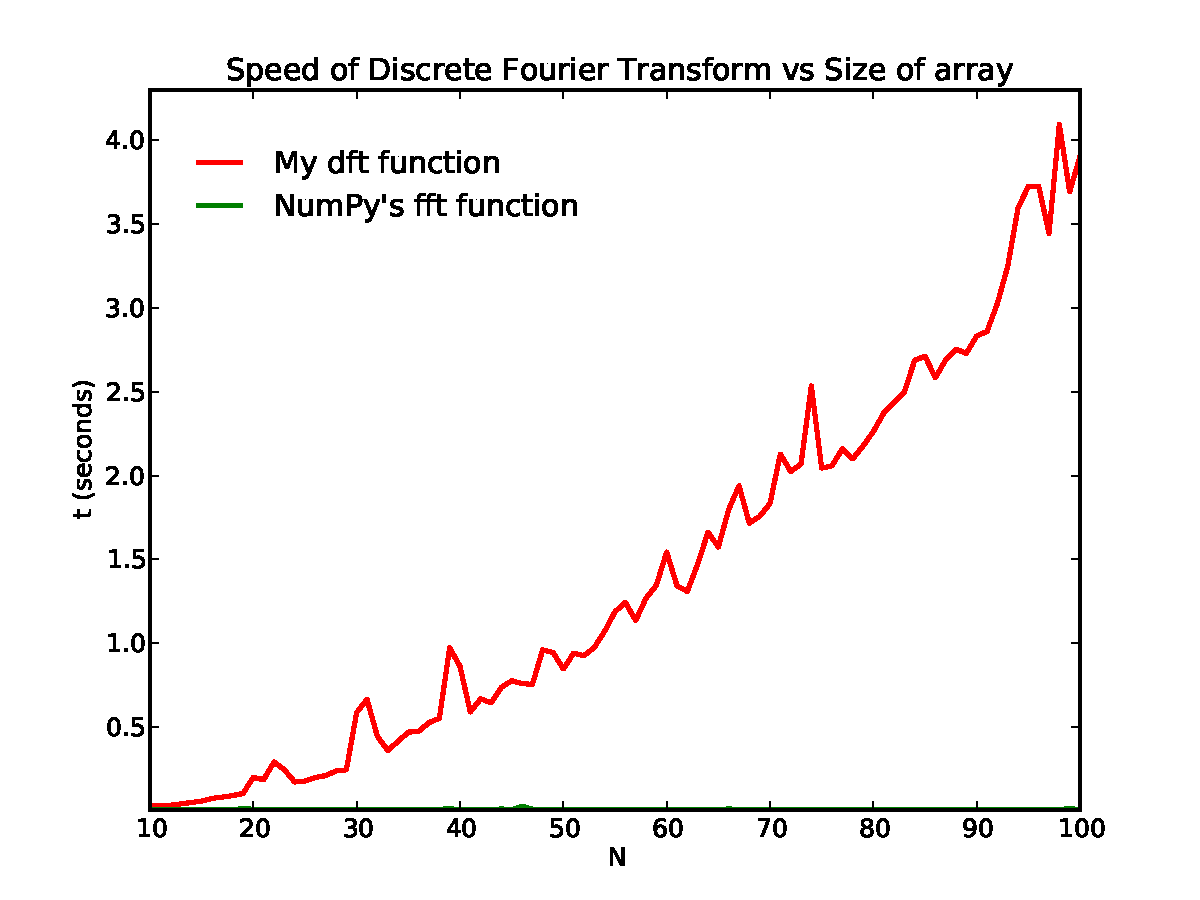
\includegraphics[width=0.6\textwidth]{ws6-b.pdf}
\caption{Performance of My dft and NumPy's fft}
\label{fig:6b}
\end{figure}

It is visually clear that for my function, the time increases as $N^2$ (e.g. 
double $N$ from 50 to 100, and the time $t$ goes up by a factor of 4).

\subsection*{c}

Note that it is difficult to see exactly how much faster NumPy's fast fourier
transform is because the green line in figure~\ref{fig:6b} hovers right around $t=0$.
To see it better, we plot $\log_{10} t$ vs $N$ instead, which is shown 
in figure~\ref{fig:6c}. 

\begin{figure}[bth]
\centering
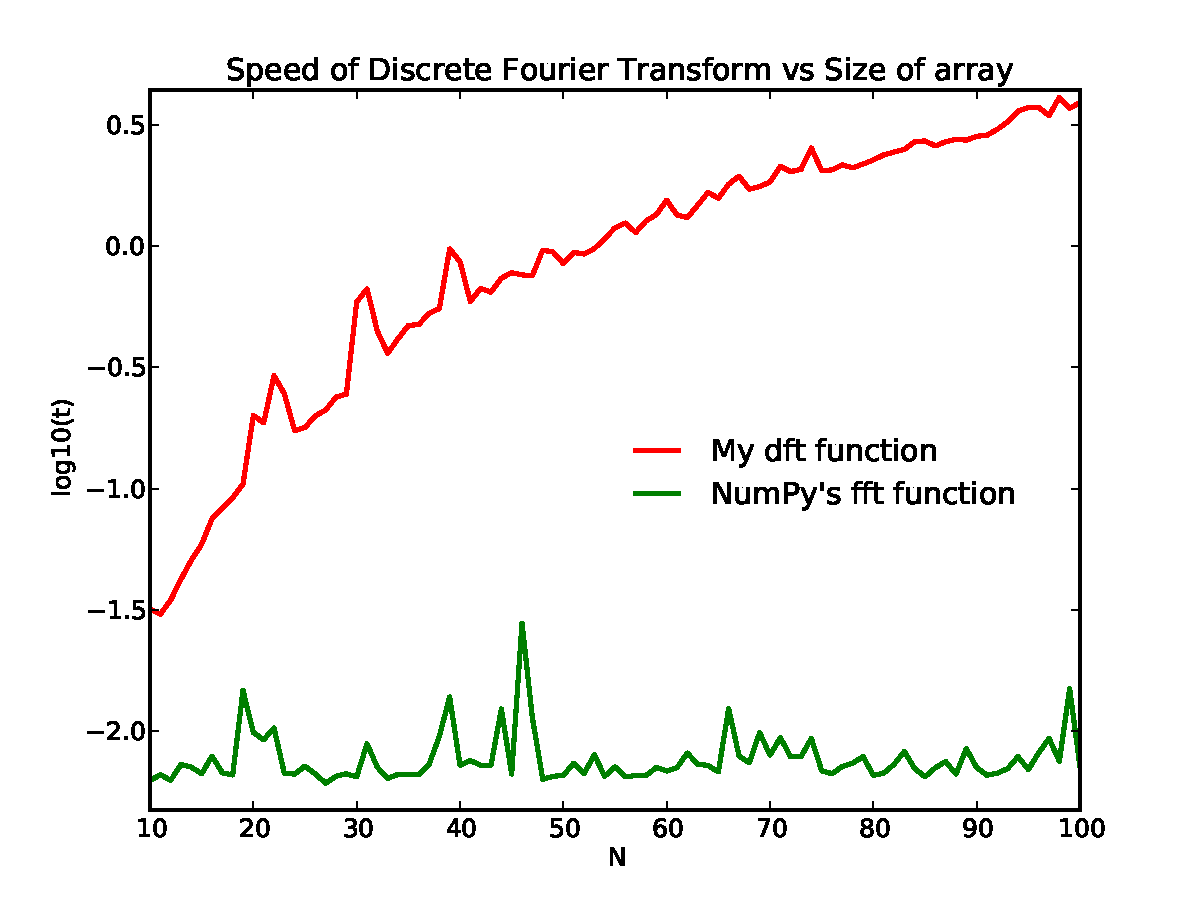
\includegraphics[width=0.6\textwidth]{ws6-c.pdf}
\caption{Same as figure~\ref{fig:6b} but with time plotted on a log scale}
\label{fig:6c}
\end{figure}

For $N$ = 100, NumPy's fast fourier transform is about 2.5 orders of magnitude 
faster than the discrete fourier transform I wrote. I'm unsure why the curve 
is so spiky, but it probably has to do with the processing power/speed of my
computer.

\end{document}